\documentclass[12pt,a4paper]{scrartcl}

\usepackage[T1]{fontenc}
\usepackage[utf8]{inputenc}
\usepackage[brazil]{babel}
\usepackage{lmodern}
\usepackage[top=3cm,left=3cm,right=2cm,bottom=2cm]{geometry}
\usepackage{graphicx}
\usepackage{amsmath,amssymb}
\usepackage{booktabs}
\usepackage{multirow}
\usepackage{float}
\usepackage{microtype}
\usepackage{caption}
\usepackage{needspace}
\usepackage{etoolbox}
\usepackage[hidelinks]{hyperref}

% evita que um título de seção comece no pé da página
\pretocmd{\section}{\Needspace*{4\baselineskip}}{}{}
\pretocmd{\subsection}{\Needspace*{3\baselineskip}}{}{}

\graphicspath{{../resultados/figuras/}}

\captionsetup{labelsep=endash, font=small, justification=centering}
\setkomafont{section}{\large\sffamily\bfseries}
\setkomafont{subsection}{\normalsize\sffamily\bfseries}
\setlength{\parindent}{1.25cm}

\newcommand{\legend}[1]{\par\vspace{0.3em}{\footnotesize #1}}
\renewcommand{\contentsname}{\hfill\normalfont\sffamily\bfseries\large Sumário\hfill}

\begin{document}

% ---------------- capa ----------------
\begin{titlepage}
\centering
{Universidade Federal do Ceará\par}
{Centro de Tecnologia\par}
{Departamento de Engenharia de Teleinformática\par}
\vspace{2.5cm}
{\sffamily Alisson Jaime Sales Barros\par}
\vfill
{\sffamily\bfseries\large Projeto Final:\\[0.3em]
Detecção de anomalias em sinais de ECG via classificação de classe única\par}
\vfill
{Fortaleza\par}
{julho de 2026\par}
\end{titlepage}

% ---------------- folha de rosto ----------------
\begin{titlepage}
\centering
{\sffamily Alisson Jaime Sales Barros\par}
\vspace{3cm}
{\sffamily\bfseries\large Projeto Final:\\[0.3em]
Detecção de anomalias em sinais de ECG via classificação de classe única\par}
\vspace{1.5cm}
\hfill\begin{minipage}{0.5\textwidth}
\small Relatório do Projeto Final apresentado às disciplinas TI0097 -- Introdução ao Reconhecimento de Padrões e TI0178 -- Projeto Integrador III, ministradas pelo Prof. Dr. Guilherme de Alencar Barreto.
\end{minipage}
\vfill
{Universidade Federal do Ceará\par}
{Centro de Tecnologia\par}
{Departamento de Engenharia de Teleinformática\par}
\vspace{1cm}
{Fortaleza\par}
{julho de 2026\par}
\end{titlepage}

% ---------------- resumo ----------------
\begin{center}{\large\sffamily\bfseries Resumo}\end{center}
\noindent Este relatório trata da detecção de anomalias em batimentos de ECG como um problema de classificação de classe única, usando a base ECG5000. Os batimentos normais são as instâncias negativas e os anômalos, as positivas. De cada batimento extraem-se atributos no domínio do tempo e no domínio da frequência, e comparam-se três detectores: distância euclidiana ao centróide dos normais, distância de Mahalanobis e erro de reconstrução por PCA (autoencoder linear). Os detectores são treinados só com batimentos normais e avaliados em 100 rodadas, antes e depois da redução de dimensionalidade via PCA. O detector de Mahalanobis com atributos de tempo obteve o melhor desempenho (F1 de 0,94 e AUC de 0,96), e os atributos de tempo superaram os de frequência, o que é compatível com a natureza morfológica das anomalias da base.

\vspace{0.6em}
\noindent\textbf{Palavras-chave}: detecção de anomalias; classe única; ECG; distância de Mahalanobis; PCA.

\vspace{1cm}
\tableofcontents

\clearpage

% ================================================================
\section{Introdução}

Este é o relatório do Projeto Final das disciplinas TI0097 e TI0178. O objetivo é desenvolver e avaliar detectores de anomalias em um problema de classificação de classe única sobre biossinais, e comparar esses detectores para técnicas diferentes de extração de atributos (tempo e frequência) e antes e depois da redução de dimensionalidade via PCA.

\subsection{Biossinal e base de dados}

Foi escolhido o sinal de eletrocardiograma (ECG) e a base ECG5000, uma das mais usadas na literatura de detecção de anomalias em batimentos cardíacos. A base tem 4998 batimentos já segmentados e reamostrados para 140 amostras cada, rotulados como normais ou anômalos. No problema de classe única deste trabalho, os batimentos normais são as instâncias negativas (2919 exemplos) e os anômalos, as positivas (2079 exemplos). A Figura~\ref{fig:exemplos} mostra um batimento de cada tipo.

\begin{figure}[H]
\centering
\caption{Exemplos de batimento normal (negativo) e anômalo (positivo) da base ECG5000.}
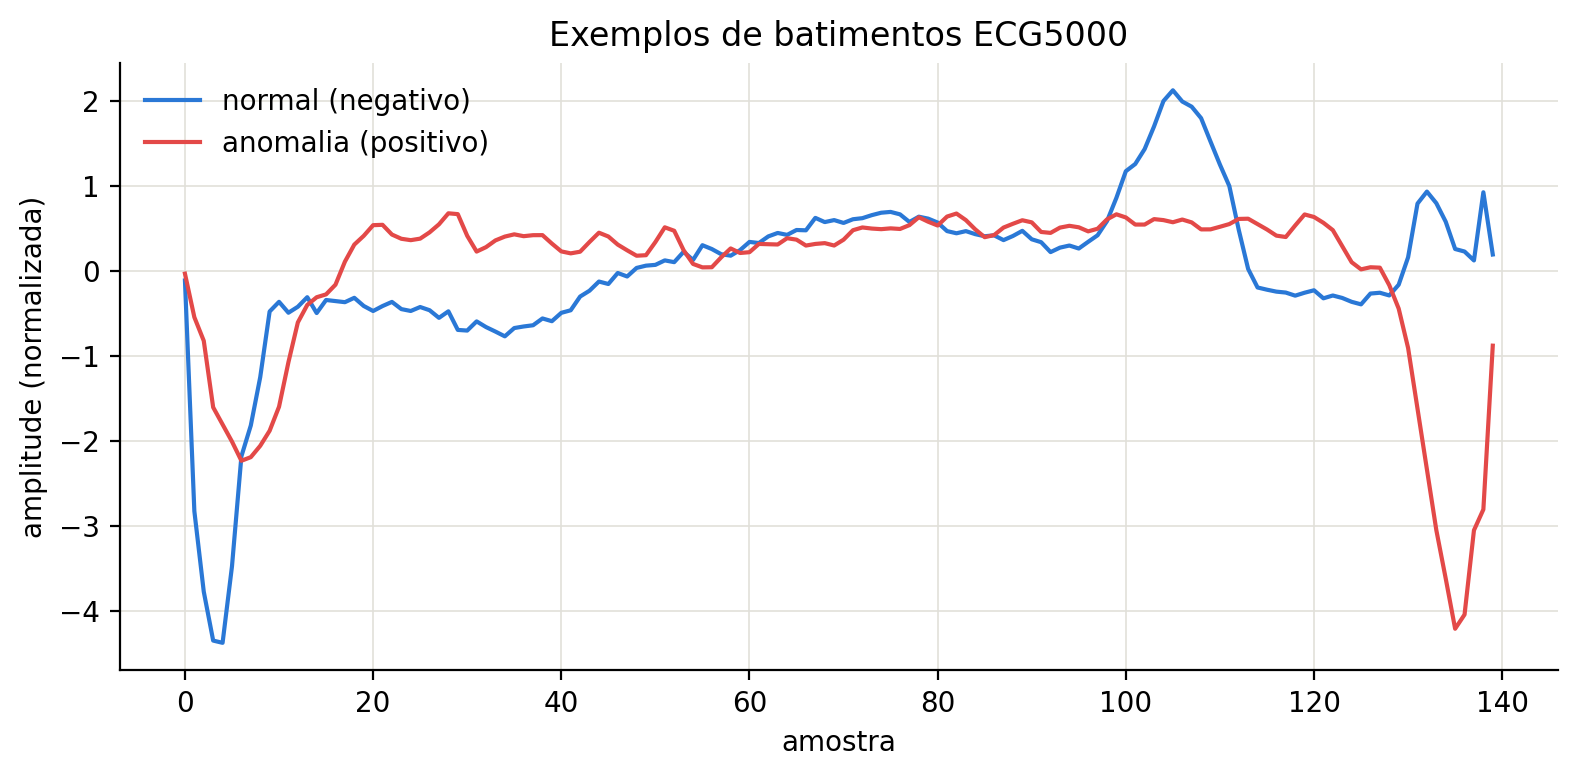
\includegraphics[width=0.75\textwidth]{exemplos_ecg.png}
\label{fig:exemplos}
\legend{Fonte: elaborada pelo autor.}
\end{figure}

Os experimentos foram feitos em Python 3 com \texttt{numpy}, \texttt{scipy} e \texttt{matplotlib}. O código está disponível em:
\begin{center}
\url{https://colab.research.google.com/drive/1KZCGpHibEiAEFDR2iO9QS4a1orlk4vfa?usp=sharing}
\end{center}

% ================================================================
\section{Extração de atributos}

De cada batimento, uma série de 140 amostras, extraiu-se um vetor de atributos, formando a matriz de dados $\mathbf{X} \in \mathbb{R}^{N \times p}$ com $N = 4998$. Para permitir a comparação pedida no enunciado, extraíram-se dois conjuntos de atributos.

No \textbf{domínio do tempo} ($p = 20$): média, desvio-padrão, variância, valor RMS, mínimo, máximo, amplitude pico-a-pico, mediana, desvio absoluto médio, assimetria, curtose, energia, variação média absoluta, taxa de cruzamentos por zero, 1º e 3º quartis, amplitude interquartílica e os três parâmetros de Hjorth (atividade, mobilidade e complexidade).

No \textbf{domínio da frequência} ($p = 15$): a partir da densidade espectral de potência (periodograma via FFT), extraíram-se potência total, centroide espectral, espalhamento espectral, entropia espectral, frequência de pico, frequência mediana, planura espectral, potência relativa em 5 bandas e máximo, média e desvio-padrão do espectro.

Os atributos foram padronizados por \emph{z-score}, com média e desvio estimados apenas no conjunto de treino de cada rodada. Como aponta o enunciado, o detector euclidiano é sensível à normalização; entre as opções testadas (sem normalização, \emph{min-max} e \emph{z-score}), a padronização \emph{z-score} deu o melhor desempenho, por colocar atributos de escalas muito diferentes, como energia e assimetria, em pé de igualdade nas distâncias.

% ================================================================
\section{Posto da matriz de dados}

Os postos das matrizes de atributos são: no domínio do tempo, $\mathbf{X}$ é $4998 \times 20$ com posto $r = 15$; no domínio da frequência, $\mathbf{X}$ é $4998 \times 15$ com posto $r = 14$. Nos dois casos o posto é menor que o número de colunas $p$, ou seja, alguns atributos são combinações lineares de outros e há redundância na representação. No conjunto de tempo, por exemplo, variância, desvio-padrão e atividade de Hjorth carregam a mesma informação; no de frequência, as potências relativas das bandas somam a unidade, o que cria uma dependência linear exata.

Esse número é útil por dois motivos. Ele indica a dimensionalidade intrínseca dos dados, ou seja, bastam $r$ atributos para representá-los sem perda, o que motiva a redução de dimensionalidade da Seção~\ref{sec:pca}. E, mais importante aqui, o posto deficiente faz a matriz de covariância dos atributos ter posto $\leq r < p$, sendo portanto singular e não invertível, o que afeta o detector de Mahalanobis e exige regularização. É o mesmo fenômeno estudado no 2º Trabalho Computacional.

% ================================================================
\section{Detectores sem redução de dimensionalidade}
\label{sec:detectores}

\subsection{Detectores implementados}

Cada detector calcula um escore de anomalia $s(\mathbf{x})$ e o compara a um limiar $\tau$; se $s(\mathbf{x}) > \tau$, a instância é classificada como anomalia.

O detector de \textbf{distância euclidiana} usa a distância euclidiana quadrática ao centróide $\mathbf{m}$ dos dados normais de treino, $s(\mathbf{x}) = \|\mathbf{x} - \mathbf{m}\|^2$.

O detector de \textbf{distância de Mahalanobis} usa $s(\mathbf{x}) = (\mathbf{x}-\mathbf{m})^{\top}\mathbf{C}^{-1}(\mathbf{x}-\mathbf{m})$, com $\mathbf{C}$ igual à matriz de covariância dos dados normais de treino. Como $\mathbf{C}$ é singular (Seção anterior), aplicou-se a regularização de Tikhonov $\mathbf{C} + \lambda\mathbf{I}$, com o menor $\lambda$ que torna a matriz bem-condicionada, o mesmo mecanismo do 2º Trabalho Computacional.

O detector de \textbf{PCA (autoencoder linear)} projeta a instância centrada no subespaço dos $q$ primeiros componentes principais dos dados normais e a reconstrói; o escore é o erro de reconstrução quadrático $s(\mathbf{x}) = \|\mathbf{x} - \hat{\mathbf{x}}\|^2$. Reteve-se o número de componentes correspondente a 95\% da variância ($q = 9$ para os atributos de tempo). Anomalias, por não pertencerem ao subespaço aprendido com os dados normais, tendem a ter erro de reconstrução alto.

\subsection{Limiar de anomalia}

Seguindo o enunciado, o limiar $\tau$ de cada detector foi definido como o percentil 95 dos escores das instâncias de treino, isto é, a distância quadrática para os detectores de distância ou o erro de reconstrução quadrático para o PCA. Isso equivale a admitir 5\% de falsos positivos sobre os dados normais de treino.

\subsection{Protocolo experimental}

Foram feitas $N_r = 100$ rodadas independentes. Em cada rodada, 80\% dos batimentos normais foram usados para treinar os detectores e definir o limiar; os 20\% restantes dos normais, junto com todas as anomalias, formaram o conjunto de teste. Como positivo é anomalia, a sensibilidade mede a fração de anomalias detectadas e a especificidade, a fração de batimentos normais classificados corretamente.

\subsection{Resultados}

A Tabela~\ref{tab:t1} traz as figuras de mérito médias, com desvio-padrão, das 100 rodadas, para os dois domínios de atributos.

\begin{table}[H]
\centering
\caption{Resultados médios (100 rodadas) dos detectores sem redução de dimensionalidade.}
\label{tab:t1}
\footnotesize
\resizebox{\textwidth}{!}{%
\begin{tabular}{llcccccc}
\toprule
Atributos & Detector & Acurácia & Sensib. & Especif. & Precisão & F1 & Tempo (ms) \\
\midrule
\multirow{3}{*}{Tempo}
 & Euclidiana  & $0{,}719 \pm 0{,}009$ & $0{,}654 \pm 0{,}014$ & $0{,}950 \pm 0{,}010$ & $0{,}979 \pm 0{,}004$ & $0{,}784 \pm 0{,}009$ & $1{,}1$ \\
 & Mahalanobis & $0{,}908 \pm 0{,}005$ & $0{,}897 \pm 0{,}009$ & $0{,}949 \pm 0{,}010$ & $0{,}984 \pm 0{,}003$ & $0{,}938 \pm 0{,}004$ & $7{,}4$ \\
 & PCA ($q{=}9$) & $0{,}598 \pm 0{,}022$ & $0{,}500 \pm 0{,}029$ & $0{,}949 \pm 0{,}009$ & $0{,}972 \pm 0{,}004$ & $0{,}660 \pm 0{,}026$ & $5{,}1$ \\
\midrule
\multirow{3}{*}{Frequência}
 & Euclidiana  & $0{,}238 \pm 0{,}002$ & $0{,}039 \pm 0{,}002$ & $0{,}949 \pm 0{,}011$ & $0{,}732 \pm 0{,}037$ & $0{,}073 \pm 0{,}003$ & $0{,}9$ \\
 & Mahalanobis & $0{,}341 \pm 0{,}009$ & $0{,}171 \pm 0{,}014$ & $0{,}948 \pm 0{,}011$ & $0{,}921 \pm 0{,}011$ & $0{,}288 \pm 0{,}020$ & $6{,}7$ \\
 & PCA ($q{=}6$) & $0{,}336 \pm 0{,}008$ & $0{,}164 \pm 0{,}011$ & $0{,}948 \pm 0{,}011$ & $0{,}919 \pm 0{,}014$ & $0{,}279 \pm 0{,}016$ & $3{,}8$ \\
\bottomrule
\end{tabular}}
\legend{Fonte: elaborada pelo autor.}
\end{table}

\subsubsection{Discussão}

A especificidade ficou perto de 95\% em todos os casos, o que é consequência direta do limiar (percentil 95 sobre os normais). O que separa os detectores é a sensibilidade, a capacidade de flagrar anomalias. Nesse ponto o Mahalanobis é o melhor, pois normaliza as distâncias pela covariância dos dados normais e leva em conta as correlações entre atributos; o euclidiano trata os atributos como independentes e de igual peso, sendo menos eficaz; e o detector por PCA ficou abaixo, o que indica que várias anomalias ainda são bem reconstruídas pelo subespaço principal dos normais.

O tipo de atributo teve forte efeito: os de tempo superaram os de frequência (F1 de 0,94 contra 0,29 no melhor detector). Isso combina com a base, cujas anomalias são morfológicas, alterações no formato e na amplitude do batimento, bem captadas por atributos temporais, mas pouco distinguíveis no espectro de potência global, que descarta a informação de forma da onda.

Em todas as figuras de mérito o melhor detector foi o de Mahalanobis com atributos de tempo (acurácia 90,8\%, sensibilidade 89,7\%, F1 0,938). Em tempo de execução, o mais rápido foi o euclidiano (cerca de 1~ms), por só calcular um centróide; o Mahalanobis é cerca de 7 vezes mais lento, por causa da estimação e inversão da covariância, mas seu custo absoluto de poucos milissegundos por rodada é aceitável, o que o mantém como melhor detector no conjunto.

Sobre a inversão da matriz de covariância: como o posto de $\mathbf{X}$ é deficiente, a covariância dos dados normais é singular. O problema foi resolvido com a regularização de Tikhonov ($\mathbf{C} + \lambda\mathbf{I}$), com $\lambda$ igual ao menor valor, em potências de 10 a partir de uma fração do traço, que eleva o recíproco do número de condicionamento acima de $10^{-10}$. Isso adiciona uma pequena constante à diagonal, completa o posto e estabiliza a inversão, sem alterar muito a geometria dos dados.

% ================================================================
\section{Detectores com redução de dimensionalidade via PCA}
\label{sec:pca}

Nesta etapa só os detectores de distância foram avaliados, com PCA como redutor de dimensionalidade sobre os atributos de tempo, o melhor domínio da seção anterior. Escolheu-se o número de componentes $q$ que preserva ao menos 95\% da variância, usando o conjunto de treino da primeira rodada. A Figura~\ref{fig:ve} mostra a variância explicada acumulada $VE(q)$.

\begin{figure}[H]
\centering
\caption{Variância explicada acumulada $VE(q)$ em função do número de componentes.}
\includegraphics[width=0.7\textwidth]{atv6_variancia_explicada.png}
\label{fig:ve}
\legend{Fonte: elaborada pelo autor.}
\end{figure}

A $VE(q)$ satura em 100\% já em $q = 15$, exatamente o posto da matriz, pois as 5 direções restantes têm variância nula. O valor escolhido foi $q = 9$, que preserva 96,8\% da variância. A Tabela~\ref{tab:t2} traz os resultados com a redução.

\begin{table}[H]
\centering
\caption{Resultados médios (100 rodadas) dos detectores de distância com redução PCA ($q = 9$).}
\label{tab:t2}
\footnotesize
\begin{tabular}{lcccccc}
\toprule
Detector & Acurácia & Sensib. & Especif. & Precisão & F1 & Tempo (ms) \\
\midrule
Euclidiana+PCA  & $0{,}712 \pm 0{,}010$ & $0{,}645 \pm 0{,}016$ & $0{,}950 \pm 0{,}011$ & $0{,}979 \pm 0{,}004$ & $0{,}777 \pm 0{,}010$ & $0{,}9$ \\
Mahalanobis+PCA & $0{,}916 \pm 0{,}003$ & $0{,}906 \pm 0{,}006$ & $0{,}949 \pm 0{,}009$ & $0{,}985 \pm 0{,}003$ & $0{,}944 \pm 0{,}002$ & $4{,}0$ \\
\bottomrule
\end{tabular}
\legend{Fonte: elaborada pelo autor.}
\end{table}

A dimensão escolhida foi $q = 9$ componentes, o que corresponde a preservar cerca de 96,8\% da variância original dos atributos de tempo. Não houve piora; ao contrário, houve leve melhora. Para o Mahalanobis, a F1 subiu de 0,938 para 0,944 e a acurácia de 90,8\% para 91,6\%, e o euclidiano manteve praticamente o mesmo desempenho. Além disso, o tempo de execução do Mahalanobis quase caiu à metade (de 7,4~ms para 4,0~ms), por operar em dimensão menor. A melhora do Mahalanobis se explica porque a redução PCA elimina as direções de variância quase nula responsáveis pela singularidade da covariância; a projeção funciona, na prática, como uma regularização, e dá uma estimativa de covariância mais estável no subespaço retido.

% ================================================================
\section{Curva ROC do melhor detector}

A Figura~\ref{fig:roc} traz a curva ROC do melhor detector, o de Mahalanobis com atributos de tempo, obtida variando o limiar $\tau$ ao longo de toda a faixa de escores.

\begin{figure}[H]
\centering
\caption{Curva ROC do detector de Mahalanobis (atributos de tempo).}
\includegraphics[width=0.62\textwidth]{atv7_roc.png}
\label{fig:roc}
\legend{Fonte: elaborada pelo autor.}
\end{figure}

A área sob a curva foi $\mathrm{AUC} = 0{,}962$, próxima de 1, o que confirma a boa capacidade de separação do detector: a curva sobe rápido e chega a sensibilidade acima de 90\% com taxa de falsos positivos abaixo de 5\%. A ROC também mostra que o ponto de operação usado nas Tabelas \ref{tab:t1} e \ref{tab:t2} (percentil 95, ou seja, falsos positivos perto de 5\%) fica na região de joelho da curva, um bom equilíbrio entre sensibilidade e especificidade.

% ================================================================
\section{Conclusão}

O problema de detectar batimentos anômalos de ECG foi formulado como classificação de classe única, com a base ECG5000. A técnica de extração de atributos foi determinante: os atributos de tempo superaram os de frequência (F1 0,94 contra 0,29), por captarem as alterações morfológicas que caracterizam as anomalias. Entre os detectores, o de Mahalanobis foi o melhor em todas as figuras de mérito, acima do euclidiano, que ignora correlações, e do baseado em PCA; o euclidiano foi o mais rápido, mas o custo do Mahalanobis é aceitável. O posto deficiente da matriz de dados tornou a covariância singular, e a inversão foi viabilizada pela regularização de Tikhonov, retomando o conteúdo do 2º Trabalho Computacional. A redução de dimensionalidade via PCA ($q = 9$, 96,8\% da variância) não piorou o desempenho, e ainda reduziu o tempo de execução, por remover as direções redundantes que atrapalhavam a estimação da covariância. O melhor detector alcançou $\mathrm{AUC} = 0{,}962$.

% ----------------------------------------------------------------
\begin{thebibliography}{9}

\bibitem{ecg5000}
GOLDBERGER, A.~L. \emph{et al.}
PhysioBank, PhysioToolkit, and PhysioNet: Components of a New Research Resource for Complex Physiologic Signals.
\emph{Circulation}, v. 101, n. 23, p. e215--e220, 2000. Base ECG5000 do \emph{UCR Time Series Classification Archive}.

\bibitem{chandola2009}
CHANDOLA, V.; BANERJEE, A.; KUMAR, V.
Anomaly Detection: A Survey. \emph{ACM Computing Surveys}, v. 41, n. 3, p. 1--58, 2009.

\bibitem{barreto-slides}
BARRETO, G.~A.
\emph{Introdução à Classificação de Padrões} (notas de aula). Fortaleza: UFC/DETI, 2026.

\end{thebibliography}

\end{document}
